\documentclass[12pt, letterpaper]{article}
\usepackage{graphicx} % Required for inserting images
\usepackage{hyperref}
\usepackage{listings}
\usepackage{amssymb}
\usepackage{amsmath}
\usepackage[english]{babel}
\usepackage{nicefrac, xfrac}
\usepackage{mathtools}
\usepackage[table,xcdraw]{xcolor}
\definecolor{light-gray}{gray}{0.95}
\definecolor{sap}{RGB}{130, 36, 51}
\definecolor{lg}{RGB}{102, 161, 95}
\usepackage[paper=a4paper,left=20mm,right=20mm,bottom=25mm,top=25mm]{geometry}
\newcommand{\code}[1]{\colorbox{light-gray}{\texttt{#1}}}
\newcommand{\codee}[1]{\colorbox{white}{\texttt{#1}}}
\newcommand{\acc}{\\\hphantom{}\\}
\newcommand{\dete}{{\rightarrow}}
\newcommand{\fdot}{{\(\bullet\) }}
\newcommand{\boxedMath}[1]{\begin{tabular}{|c|}\hline \texttt{#1} \\ \hline\end{tabular} :}
\title{Azienda 1}
\author{Marco Casu}
\date{\vspace{-5ex}}
\begin{document}



\maketitle
\begin{figure}[h]
    \centering{
    
    }
\end{figure}
\section{Requisiti}
\begin{enumerate}
    \item Un \underline{Impiegato} avrà ad esso associato i record riguardanti i suoi 
    dati personali, ossia nome, data di nascita, cognome, e stipendio.
    \item Ogni \underline{Impiegato} inoltre avrà un altro dato associato, ossia la data nella 
    quale ha iniziato a lavorare nel \underline{Dipartimento} alla quale afferisce.
    \item Tale campo è dinamico in quanto potrebbe variare in correlazione ad eventuali 
    cambi di \underline{Dipartimento}.
    \item Di ogni \underline{Dipartimento} vi saranno in egual modo i record con i dati menzionati 
    associati, ossia nome e numero del centralino.
    \item Ogni \underline{Impiegato} sarà in relazione con un \underline{Dipartimento}.
    \item Ogni \underline{Dipartimento} sarà in una relazione esclusiva con un certo 
    \underline{Impiegato}, che ne sarà il direttore. 
    \item Uno \underline{Impiegato} può essere direttore di un \underline{Dipartimento} 
    indipendentemente dal dipartimento alla quale afferisce.
    \item Uno stesso \underline{Impiegato} può dirigere più di un \underline{Dipartimento} .
    \item Ogni \underline{Impiegato} può partecipare a più \underline{Progetti}. 
    \item Un apposita entità \underline{Partecipazione} si occuperà di tale relazione, specificando 
    anche la data nella quale l'\underline{Impiegato} ha iniziato a lavorare a tale 
    \underline{Progetto}.
    \item Un \underline{Progetto} avrà ad esso associato i record riguardanti i suoi 
    dettagli, come il nome ed il budget.
    \item Un  \underline{Impiegato}, nell'implementazione, potrà avere più dipartimenti alla quale 
    afferisce, lo scopo di ciò, è dare uno storico dei dipartimenti 
    passati alla quale è stato associato, difatti per ogni associazione fra  \underline{Impiegato} e \underline{Dipartimento},
    vi sarà una data di inizio-contratto in quel \underline{Dipartimento}.
    \item Come di facile intuizione, l'associazione con la data più recente sarà considerata 
    quella valida/corrente.
\end{enumerate}
\newpage
\section{Diagramma UML}
\begin{center}
    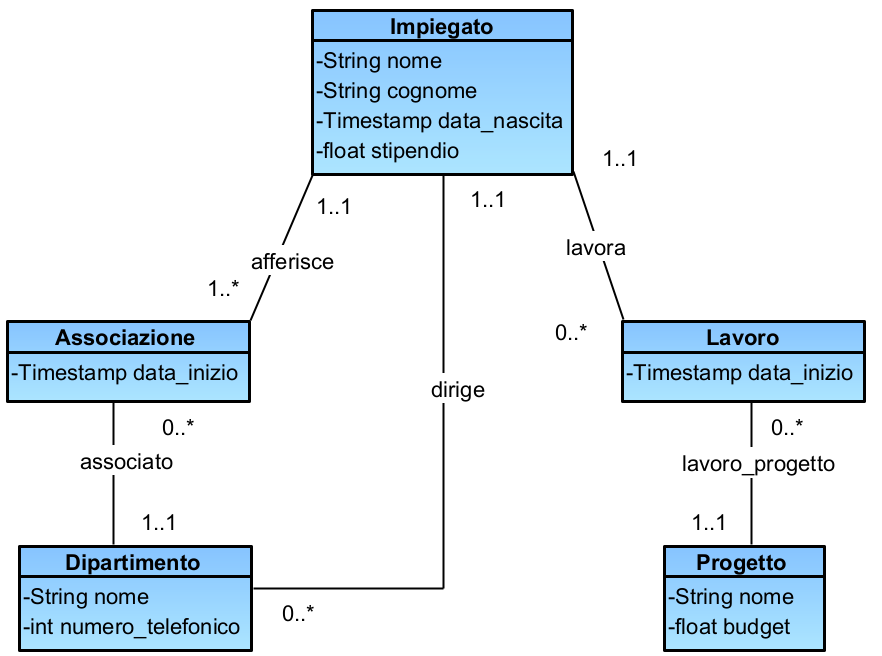
\includegraphics[width=1\textwidth ]{images/UML_visualParadigm.png}
\end{center}
\end{document}
